% Options for packages loaded elsewhere
\PassOptionsToPackage{unicode}{hyperref}
\PassOptionsToPackage{hyphens}{url}
\PassOptionsToPackage{dvipsnames,svgnames,x11names}{xcolor}
\PassOptionsToPackage{space}{xeCJK}
\documentclass[
  10pt,
]{article}
\usepackage{xcolor}
\usepackage[margin=0.65in]{geometry}
\usepackage{amsmath,amssymb}
\setcounter{secnumdepth}{-\maxdimen} % remove section numbering
\usepackage{iftex}
\ifPDFTeX
  \usepackage[T1]{fontenc}
  \usepackage[utf8]{inputenc}
  \usepackage{textcomp} % provide euro and other symbols
\else % if luatex or xetex
  \usepackage{unicode-math} % this also loads fontspec
  \defaultfontfeatures{Scale=MatchLowercase}
  \defaultfontfeatures[\rmfamily]{Ligatures=TeX,Scale=1}
\fi
\usepackage{lmodern}
\ifPDFTeX\else
  % xetex/luatex font selection
  \setmainfont[]{Arial}
  \setmonofont[]{Consolas}
  \ifXeTeX
    \usepackage{xeCJK}
    \setCJKmainfont[]{Microsoft YaHei}
  \fi
  \ifLuaTeX
    \usepackage[]{luatexja-fontspec}
    \setmainjfont[]{Microsoft YaHei}
  \fi
\fi
% Use upquote if available, for straight quotes in verbatim environments
\IfFileExists{upquote.sty}{\usepackage{upquote}}{}
\IfFileExists{microtype.sty}{% use microtype if available
  \usepackage[]{microtype}
  \UseMicrotypeSet[protrusion]{basicmath} % disable protrusion for tt fonts
}{}
\makeatletter
\@ifundefined{KOMAClassName}{% if non-KOMA class
  \IfFileExists{parskip.sty}{%
    \usepackage{parskip}
  }{% else
    \setlength{\parindent}{0pt}
    \setlength{\parskip}{6pt plus 2pt minus 1pt}}
}{% if KOMA class
  \KOMAoptions{parskip=half}}
\makeatother
\usepackage{longtable,booktabs,array}
\usepackage{calc} % for calculating minipage widths
% Correct order of tables after \paragraph or \subparagraph
\usepackage{etoolbox}
\makeatletter
\patchcmd\longtable{\par}{\if@noskipsec\mbox{}\fi\par}{}{}
\makeatother
% Allow footnotes in longtable head/foot
\IfFileExists{footnotehyper.sty}{\usepackage{footnotehyper}}{\usepackage{footnote}}
\makesavenoteenv{longtable}
\usepackage{graphicx}
\makeatletter
\newsavebox\pandoc@box
\newcommand*\pandocbounded[1]{% scales image to fit in text height/width
  \sbox\pandoc@box{#1}%
  \Gscale@div\@tempa{\textheight}{\dimexpr\ht\pandoc@box+\dp\pandoc@box\relax}%
  \Gscale@div\@tempb{\linewidth}{\wd\pandoc@box}%
  \ifdim\@tempb\p@<\@tempa\p@\let\@tempa\@tempb\fi% select the smaller of both
  \ifdim\@tempa\p@<\p@\scalebox{\@tempa}{\usebox\pandoc@box}%
  \else\usebox{\pandoc@box}%
  \fi%
}
% Set default figure placement to htbp
\def\fps@figure{htbp}
\makeatother
\setlength{\emergencystretch}{3em} % prevent overfull lines
\providecommand{\tightlist}{%
  \setlength{\itemsep}{0pt}\setlength{\parskip}{0pt}}
\usepackage{bookmark}
\IfFileExists{xurl.sty}{\usepackage{xurl}}{} % add URL line breaks if available
\urlstyle{same}
\hypersetup{
  colorlinks=true,
  linkcolor={Maroon},
  filecolor={Maroon},
  citecolor={Blue},
  urlcolor={blue},
  pdfcreator={LaTeX via pandoc}}

\author{}
\date{}

\usepackage{float}
\usepackage{needspace}
\Urlmuskip=0mu plus 2mu\relax
\begin{document}

\section{Data integration, degradation audit, and new training
results}\label{data-integration-degradation-audit-and-new-training-results}

November 13, 2026 · Eye Sentinel

\href{training-results.zh.md}{中文} ·
\href{training-results.en.pdf}{English PDF} ·
\href{../progress-overview.en.md}{Daily progress overview}

\subsection{What this round completed}\label{what-this-round-completed}

This report follows the same-day
\href{../data-review/data-and-degradation-review.en.md}{data and
degradation review} and records the allocation, training, and
development evaluation of the audited images. The
\href{../experimental-analysis/experimental-analysis.en.md}{experimental
analysis} examines source differences, sampling, and checkpoint
selection in more detail.

The fixed expanded\_20261113 release combines the additions with the
original disease cohort. Four EfficientNet-B0 arms start from the same
ImageNet pretrained initialization and compare original data, expanded
data, and expanded data with 30\% or 50\% degradation. Each completes
1,200 optimizer updates, or parameter adjustments, ending at that budget
within the configuration's 20-epoch ceiling. Model validation selects
checkpoints, while rule development supports post-training analysis and
subsequent manual-review design. All arms use seed 20261113.

AUROC is the area under the receiver operating characteristic curve. It
represents the probability that a randomly selected positive image
scores above a randomly selected negative, with ties counting as half. A
value of 0.5 corresponds to random ranking and 1 to complete separation.
Misses and false positives are evaluated separately at specified
screening thresholds.

The opening results use each arm's validation-selected checkpoint:
update 300 for expanded clean and update 1,200 for the other arms. The
matched update-1,200 comparison appears under ``Additional check of
checkpoint selection'' and is also used in the daily overview and
experimental analysis.

On the 305-image ODIR rule-development subset, with 28 positives, AUROC
was 0.9712 for original-data training and 0.9323 for expanded-data
training. The 30\% and 50\% degradation arms achieved 0.9281 and 0.9404.
At the common display threshold of 0.5, misses among 12 real
poor-quality positives were 5, 0, 0, 0, respectively. Expansion improves
detection of these 12 poor-quality positives while reducing ranking on
original ODIR photographs. The source-specific results and
miss/false-positive counts below explain both changes.

On the 153-image KEH optic-disc-crop development subset, with 75
positives, the four AUROCs were 0.6627, 0.9212, 0.9321, 0.9368,
respectively. KEH mainly contains optic-disc crops, with a different
field of view from full fundus photographs. ODIR's 28 positive images
form 19 confirmed positive linked groups; paired eyes and associated
images in a group are handled together in statistical resampling.

\subsection{Data integration and the additional
finding}\label{data-integration-and-the-additional-finding}

The joint disease manifest contains 24,491 images. SHA256 checks image
content, and full RGB decoding confirms that each image can be read.
Every image passed these checks, and all 9,070 additions match the pixel
identities recorded during the source review. Patient, same-eye,
photograph-variant, and confirmed cross-source associations were
combined before allocation. No linked group or identical decoded RGB
image crosses roles. All 386 known patient identifiers have one role.
Sources without patient identifiers are grouped by confirmed image
relationships; their recorded group counts describe image groups.

Rebuilding the association graph independently found 18 original disease
images linked to official EyeQ test groups. The new release removes 16
training and two model-validation images, and applies the existing
12-image rule-development repair. The same exclusions apply to the
original-data control and all expanded arms. Historical models trained
before this removal; subsequent evaluation involving these EyeQ groups
uses this round's models.

\Needspace{12\baselineskip}
\begin{longtable}[]{@{}
  >{\raggedright\arraybackslash}p{(\linewidth - 6\tabcolsep) * \real{0.2000}}
  >{\raggedleft\arraybackslash}p{(\linewidth - 6\tabcolsep) * \real{0.2667}}
  >{\raggedleft\arraybackslash}p{(\linewidth - 6\tabcolsep) * \real{0.2667}}
  >{\raggedleft\arraybackslash}p{(\linewidth - 6\tabcolsep) * \real{0.2667}}@{}}
\toprule\noalign{}
\begin{minipage}[b]{\linewidth}\raggedright
Role
\end{minipage} & \begin{minipage}[b]{\linewidth}\raggedleft
Original images / positives
\end{minipage} & \begin{minipage}[b]{\linewidth}\raggedleft
Additive images / positives
\end{minipage} & \begin{minipage}[b]{\linewidth}\raggedleft
Total images / positives
\end{minipage} \\
\midrule\noalign{}
\endhead
\bottomrule\noalign{}
\endlastfoot
Training & 10,338 / 4,409 & 5,142 / 1,996 & 15,480 / 6,405 \\
Model validation & 1,188 / 487 & 858 / 336 & 2,046 / 823 \\
Rule development & 1,220 / 503 & 833 / 311 & 2,053 / 814 \\
Internal and new reserved tests & 1,233 / 489 & 2,237 / 803 & 3,470 /
1,292 \\
\end{longtable}

ACRIMA's 705 images/396 positives and HYGD's 737 images/540 positives
also retain their external-test roles. All 420 PAPILA images are held
out as a complete source; its 87 positive images represent 47 known
positive patients. The 105 official test images propagate test
assignment to their entire linked groups. The 204 suspect images are
retained separately; binary disease supervision uses explicit positive
or negative labels. LAG, GRAPE, FIVES, Fundus-AVSeg, and MSHF use joint
association grouping. KEH's optic-disc crop domain and source-specific
clinical versus RG referral endpoints remain explicit.

Real poor-quality positives are allocated as 72 training, 12
model-validation, 12 rule-development, and 50 test images. FIVES uses at
least one poor official quality dimension; MSHF uses official
overall-quality code 0. Their definitions remain distinct. The 12
rule-development positives comprise seven FIVES and five MSHF images.

\begin{figure}[H]
\centering
\pandocbounded{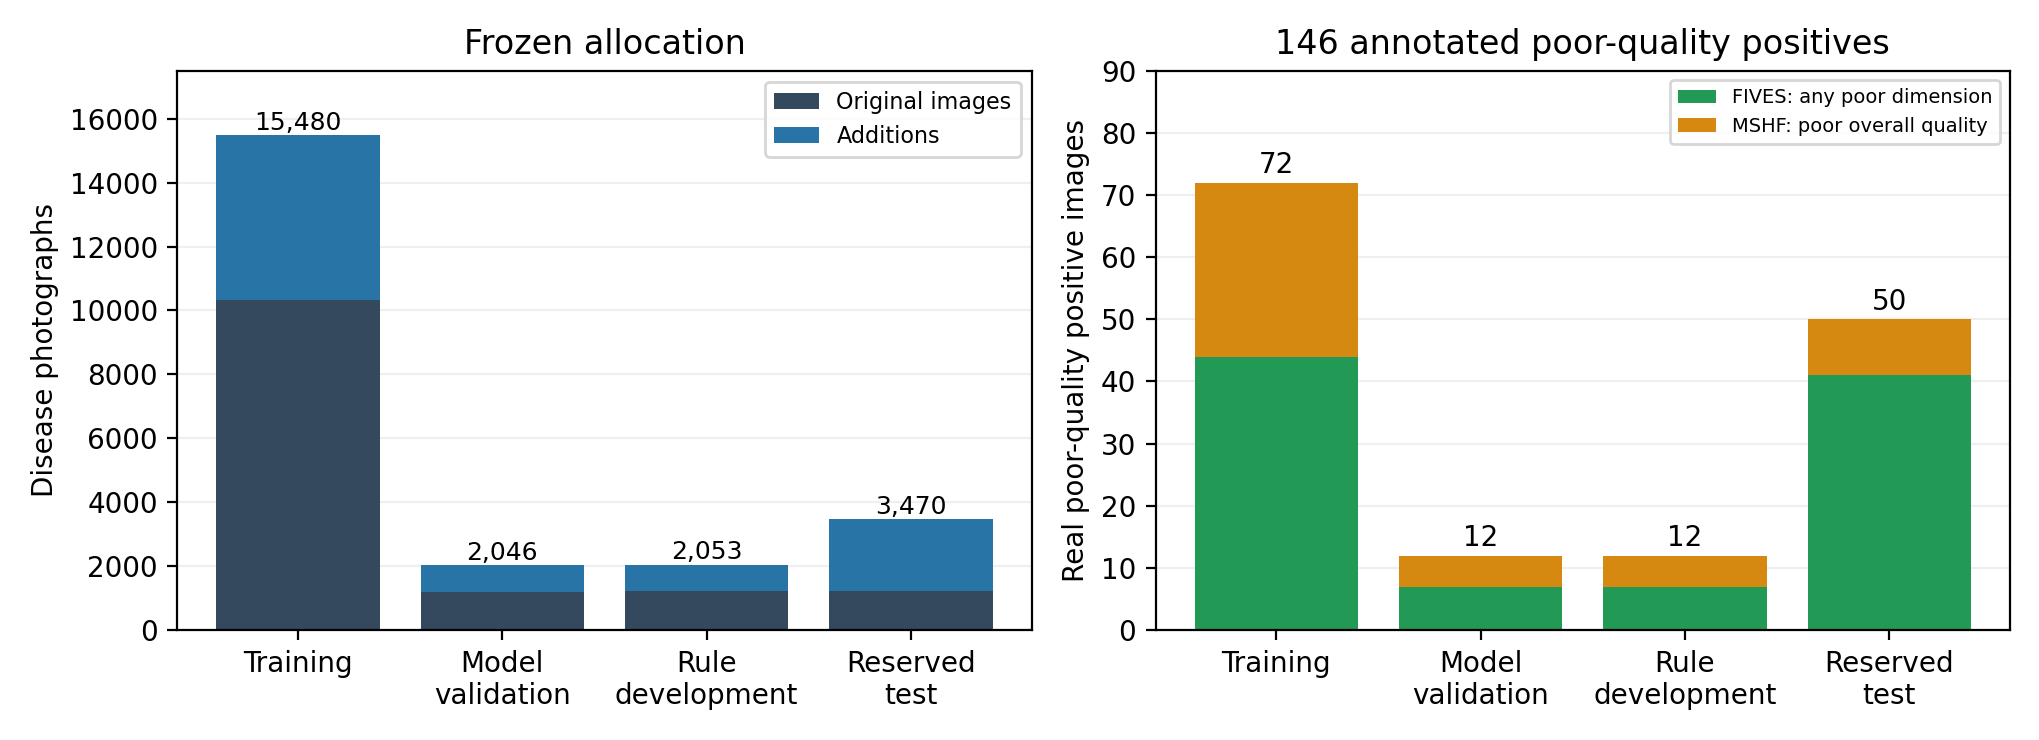
\includegraphics[keepaspectratio,alt={Frozen allocation and real poor-quality positives}]{cohort-and-quality.png}}
\caption{Frozen allocation and real poor-quality positives}
\end{figure}

Figure 1 separates original and additive images by role, covering
training, validation, development, and internal/new reserved tests.
ACRIMA and HYGD external tests are listed separately in the text. The
right panel shows the allocation of 146 real poor-quality positives by
source and role, retaining each source's official quality definition.

\subsection{Degradation algorithms and author
models}\label{degradation-algorithms-and-author-models}

Five author releases were verified: CoFe-Net, ArcNet, FD3, Catintell,
and CUNSB-RFIE. CUNSB's four checkpoints loaded with finite tensors; its
generator matched the author code and ran once on a 320×320 image. The
\href{degradation-audit.en.md}{degradation audit} records version and
execution details. This round uses the project acquisition simulator for
disease training; the author network supports a separate restoration
experiment.

Disease images are padded and resized to 320×320 before degradation and
ImageNet normalization. Each draw selects illumination changes, defocus,
or mild scatter with equal probability; defocus may add light noise or
JPEG compression. Scatter reduces local contrast through smooth
intensity mixing. Spatial blur scales with visible fundus-field
diameter. Exposure spans 0.72--1.12, reference blur radius 0.5--2.0 at a
512-pixel field, and scatter opacity 0.03--0.10. Image identity, epoch,
and seed determine replayable parameters; original black borders remain
unchanged. Degradation probability is independent of disease label.

A descriptive comparison uses 18 HRF and 120 Real Fundus same-eye pairs.
Median green-channel Laplacian-variance ratios relative to high-quality
originals are 0.516 and 0.101 for real low-quality images, versus 0.805
and 0.719 for mild synthetic defocus. This statistic describes detail
changes and also responds to noise and alignment. Quality training uses
original images and their original quality targets; degradation applies
to disease training.

\subsection{Training budget, sampling, and checkpoint
selection}\label{training-budget-sampling-and-checkpoint-selection}

All arms share the manifest, validation roles, seed 20261113, 320-pixel
inputs, batch size 16, AdamW learning rate 0.0001, and update budget.
The original-data arm filters training origins only. Each image receives
the inverse square root of its source/class image count as its sampling
weight. Smaller combinations have higher individual draw probabilities.
Adding sources changes the original sources' draw counts under this
common rule. Distinct original images actually sampled were 8339, 9830,
9830, 9830, respectively; these counts remain separate from image
variants. Realized degradation proportions were 30.1\% and 50.1\%.

Validation occurs every 300 updates. Checkpoints maximize the mean of 11
source-specific AUROCs where validation contains both classes; endpoints
are evaluated within source before averaging. Resume and worker-loading
consistency checks are retained in the supporting audit records.

\Needspace{12\baselineskip}
\begin{longtable}[]{@{}
  >{\raggedright\arraybackslash}p{(\linewidth - 8\tabcolsep) * \real{0.1579}}
  >{\raggedleft\arraybackslash}p{(\linewidth - 8\tabcolsep) * \real{0.2105}}
  >{\raggedleft\arraybackslash}p{(\linewidth - 8\tabcolsep) * \real{0.2105}}
  >{\raggedleft\arraybackslash}p{(\linewidth - 8\tabcolsep) * \real{0.2105}}
  >{\raggedleft\arraybackslash}p{(\linewidth - 8\tabcolsep) * \real{0.2105}}@{}}
\toprule\noalign{}
\begin{minipage}[b]{\linewidth}\raggedright
Arm
\end{minipage} & \begin{minipage}[b]{\linewidth}\raggedleft
Training images
\end{minipage} & \begin{minipage}[b]{\linewidth}\raggedleft
Selected update
\end{minipage} & \begin{minipage}[b]{\linewidth}\raggedleft
Mean source validation AUROC
\end{minipage} & \begin{minipage}[b]{\linewidth}\raggedleft
Real poor-quality positive misses
\end{minipage} \\
\midrule\noalign{}
\endhead
\bottomrule\noalign{}
\endlastfoot
Original data & 10,338 & 1200 & 0.9235 & 5/12 \\
Expanded data & 15,480 & 300 & 0.9513 & 0/12 \\
Expanded + 30\% & 15,480 & 1200 & 0.9622 & 0/12 \\
Expanded + 50\% & 15,480 & 1200 & 0.9632 & 0/12 \\
\end{longtable}

\begin{figure}[H]
\centering
\pandocbounded{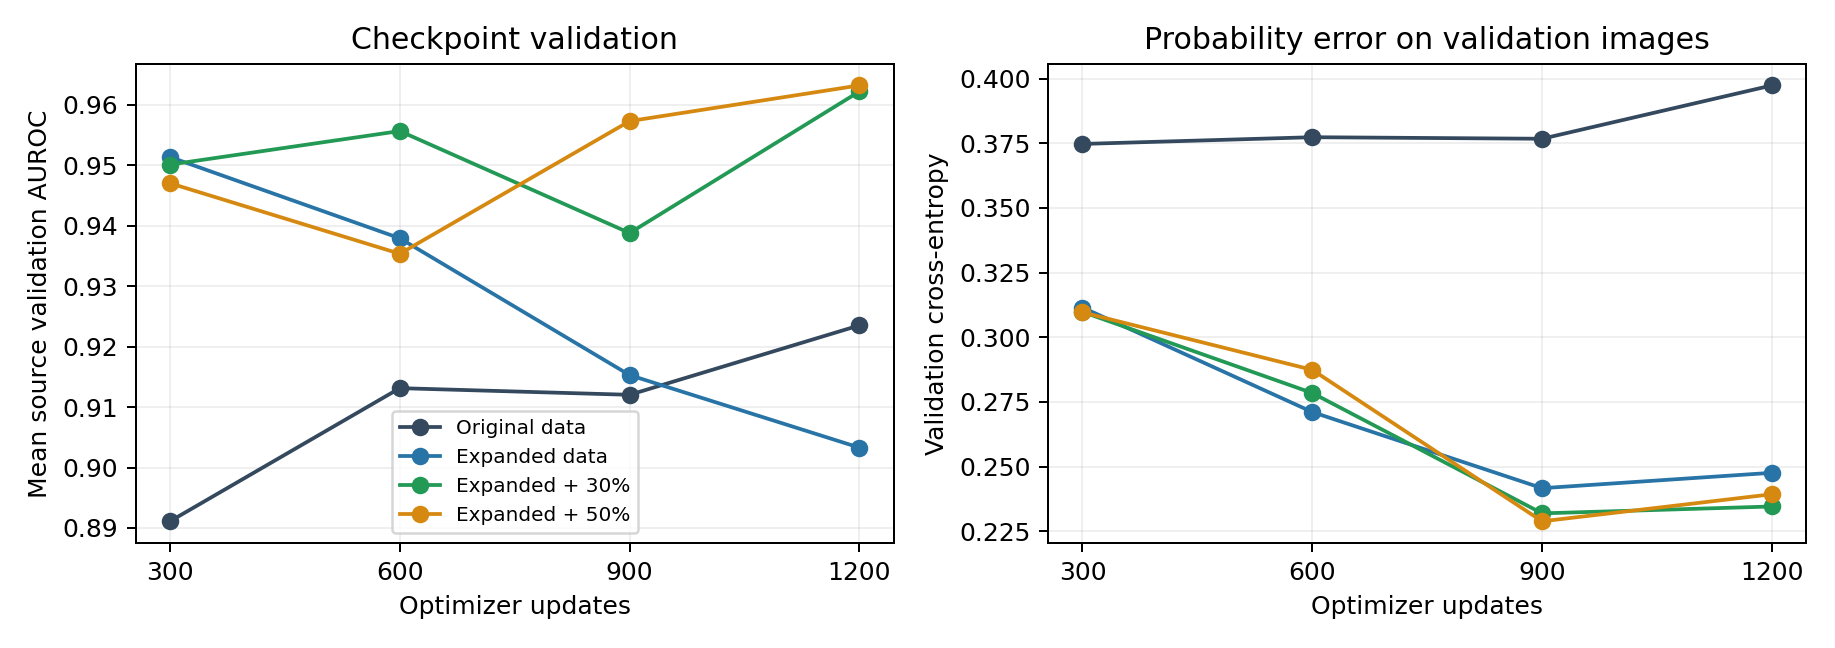
\includegraphics[keepaspectratio,alt={Validation at matched optimizer-update budgets}]{training-curves.png}}
\caption{Validation at matched optimizer-update budgets}
\end{figure}

Figure 2 shows mean source AUROC on the left and cross-entropy over
validation images on the right. Cross-entropy penalizes confident wrong
probabilities. Nodes represent 300, 600, 900, and 1,200 updates.
Expanded clean selects update 300; the other arms select update 1,200.

\subsection{Observed effects on rule-development
photographs}\label{observed-effects-on-rule-development-photographs}

The following AUROCs use each arm's selected checkpoint on the same
rule-development originals. The complete results also retain AUPRC, the
area under the precision--recall curve; Brier score, the mean squared
difference between predicted probabilities and 0/1 labels; and
calibration error. AUPRC depends on positive prevalence and is useful
for comparisons within a source. Lower Brier scores indicate smaller
probability errors.

\Needspace{12\baselineskip}
\begin{longtable}[]{@{}
  >{\raggedright\arraybackslash}p{(\linewidth - 8\tabcolsep) * \real{0.1579}}
  >{\raggedleft\arraybackslash}p{(\linewidth - 8\tabcolsep) * \real{0.2105}}
  >{\raggedleft\arraybackslash}p{(\linewidth - 8\tabcolsep) * \real{0.2105}}
  >{\raggedleft\arraybackslash}p{(\linewidth - 8\tabcolsep) * \real{0.2105}}
  >{\raggedleft\arraybackslash}p{(\linewidth - 8\tabcolsep) * \real{0.2105}}@{}}
\toprule\noalign{}
\begin{minipage}[b]{\linewidth}\raggedright
Source (images / positives)
\end{minipage} & \begin{minipage}[b]{\linewidth}\raggedleft
Original
\end{minipage} & \begin{minipage}[b]{\linewidth}\raggedleft
Expanded
\end{minipage} & \begin{minipage}[b]{\linewidth}\raggedleft
30\% degradation
\end{minipage} & \begin{minipage}[b]{\linewidth}\raggedleft
50\% degradation
\end{minipage} \\
\midrule\noalign{}
\endhead
\bottomrule\noalign{}
\endlastfoot
AIROGS (773/380) & 0.9687 & 0.9374 & 0.9583 & 0.9593 \\
ODIR (305/28) & 0.9712 & 0.9323 & 0.9281 & 0.9404 \\
Kaggle (142/95) & 0.9830 & 0.9698 & 0.9742 & 0.9718 \\
LAG (481/169) & 0.9465 & 0.9750 & 0.9844 & 0.9832 \\
KEH (153/75) & 0.6627 & 0.9212 & 0.9321 & 0.9368 \\
BEH (33/8) & 0.9100 & 0.9050 & 0.8900 & 0.9100 \\
FIVES (27/13) & 0.8736 & 0.9341 & 0.9560 & 0.9505 \\
\end{longtable}

Each arm also sets a source-specific threshold at the higher 95th
percentile of its validation-negative scores, predicting positive only
above the threshold. The table reports resulting sensitivity and
specificity on rule development, distinguishing improved detection from
a general score shift. The 95\% target is set on validation; the
development specificity in the table follows from the new case scores.
With only 14 validation negatives, the FIVES rule selects the maximum
negative score and achieves 100\% validation specificity.

\Needspace{12\baselineskip}
\begin{longtable}[]{@{}
  >{\raggedright\arraybackslash}p{(\linewidth - 8\tabcolsep) * \real{0.1579}}
  >{\raggedleft\arraybackslash}p{(\linewidth - 8\tabcolsep) * \real{0.2105}}
  >{\raggedleft\arraybackslash}p{(\linewidth - 8\tabcolsep) * \real{0.2105}}
  >{\raggedleft\arraybackslash}p{(\linewidth - 8\tabcolsep) * \real{0.2105}}
  >{\raggedleft\arraybackslash}p{(\linewidth - 8\tabcolsep) * \real{0.2105}}@{}}
\toprule\noalign{}
\begin{minipage}[b]{\linewidth}\raggedright
Source
\end{minipage} & \begin{minipage}[b]{\linewidth}\raggedleft
Original: sensitivity / specificity
\end{minipage} & \begin{minipage}[b]{\linewidth}\raggedleft
Expanded
\end{minipage} & \begin{minipage}[b]{\linewidth}\raggedleft
30\% degradation
\end{minipage} & \begin{minipage}[b]{\linewidth}\raggedleft
50\% degradation
\end{minipage} \\
\midrule\noalign{}
\endhead
\bottomrule\noalign{}
\endlastfoot
ODIR & 71.4\% / 96.4\% & 42.9\% / 97.1\% & 53.6\% / 96.0\% & 53.6\% /
96.4\% \\
AIROGS & 84.2\% / 93.6\% & 71.3\% / 93.9\% & 78.2\% / 94.1\% & 76.3\% /
94.9\% \\
FIVES & 61.5\% / 92.9\% & 61.5\% / 100.0\% & 76.9\% / 92.9\% & 92.3\% /
78.6\% \\
\end{longtable}

All 49 admitted MSHF images are positive, so same-source specificity
cannot be estimated. MSHF therefore contributes positive-detection
results, while FIVES provides both positive detection and negative false
positives.

\begin{figure}[H]
\centering
\pandocbounded{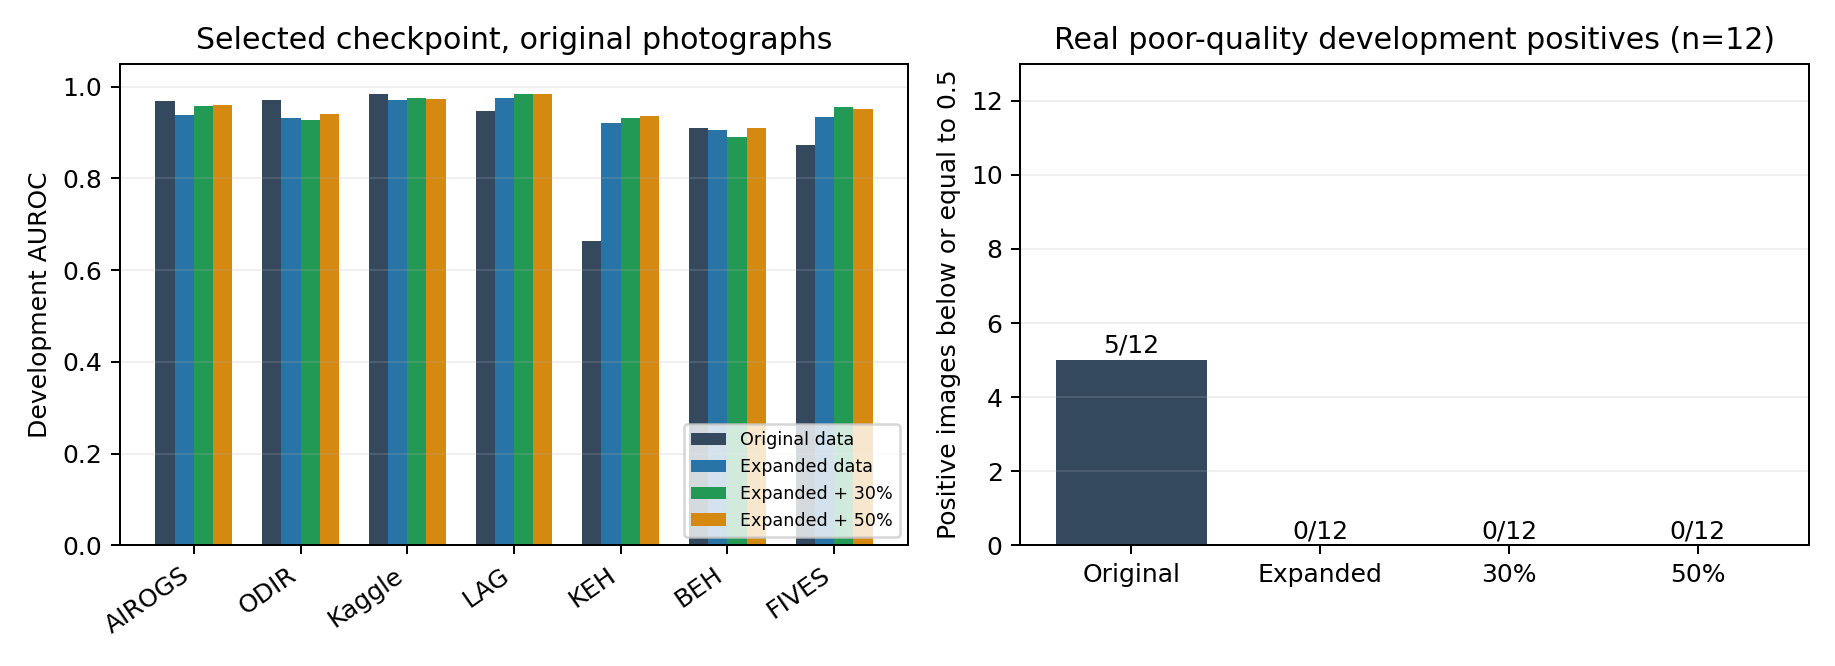
\includegraphics[keepaspectratio,alt={Original-image ranking and real poor-quality positive misses}]{development-results.png}}
\caption{Original-image ranking and real poor-quality positive misses}
\end{figure}

Figure 3 compares seven major sources on the left and misses among 12
real poor-quality positives on the right. The common 0.5 threshold
displays comparable counts; source validation thresholds are evaluated
in the preceding table. The 12 poor-quality positives comprise seven
FIVES and five MSHF images, and the combined count describes these fixed
development photographs. Disease thresholds and manual-review rules will
be chosen during subsequent development.

\Needspace{12\baselineskip}
\begin{longtable}[]{@{}
  >{\raggedright\arraybackslash}p{(\linewidth - 4\tabcolsep) * \real{0.2727}}
  >{\raggedleft\arraybackslash}p{(\linewidth - 4\tabcolsep) * \real{0.3636}}
  >{\raggedleft\arraybackslash}p{(\linewidth - 4\tabcolsep) * \real{0.3636}}@{}}
\toprule\noalign{}
\begin{minipage}[b]{\linewidth}\raggedright
Contrast (later arm minus reference)
\end{minipage} & \begin{minipage}[b]{\linewidth}\raggedleft
Sensitivity change (percentage points)
\end{minipage} & \begin{minipage}[b]{\linewidth}\raggedleft
Group-bootstrap 95\% interval
\end{minipage} \\
\midrule\noalign{}
\endhead
\bottomrule\noalign{}
\endlastfoot
Expanded − Original & +41.7 & {[}+16.7, +66.7{]} \\
30\% − Expanded & +0.0 & {[}+0.0, +0.0{]} \\
50\% − Expanded & +0.0 & {[}+0.0, +0.0{]} \\
\end{longtable}

Intervals use 2,000 paired resamples of patient/linked image groups,
comparing decisions on the same photographs. Only 12 positive images
contribute. The experiment trains one seed, and the intervals describe
case-sampling variation. Degradation and expanded clean make identical
decisions on these 12 images, producing a zero difference in every
resample. Differences in new cases require evaluation on a larger
real-quality sample.

A fixed subset of 384 rule-development originals, comprising 146
positive and 238 negative images, was selected by identity hash. It was
evaluated after defocus of radius 2 at a 512-pixel reference field and
exposure multiplication by 0.70. Each cell is the count of misses /
false positives, among 146 positives and 238 negatives respectively, at
display threshold 0.5. Each original and its two variants belong to the
same case observation.

\Needspace{12\baselineskip}
\begin{longtable}[]{@{}
  >{\raggedright\arraybackslash}p{(\linewidth - 8\tabcolsep) * \real{0.1579}}
  >{\raggedleft\arraybackslash}p{(\linewidth - 8\tabcolsep) * \real{0.2105}}
  >{\raggedleft\arraybackslash}p{(\linewidth - 8\tabcolsep) * \real{0.2105}}
  >{\raggedleft\arraybackslash}p{(\linewidth - 8\tabcolsep) * \real{0.2105}}
  >{\raggedleft\arraybackslash}p{(\linewidth - 8\tabcolsep) * \real{0.2105}}@{}}
\toprule\noalign{}
\begin{minipage}[b]{\linewidth}\raggedright
Condition
\end{minipage} & \begin{minipage}[b]{\linewidth}\raggedleft
Original: misses / false positives
\end{minipage} & \begin{minipage}[b]{\linewidth}\raggedleft
Expanded
\end{minipage} & \begin{minipage}[b]{\linewidth}\raggedleft
30\% degradation
\end{minipage} & \begin{minipage}[b]{\linewidth}\raggedleft
50\% degradation
\end{minipage} \\
\midrule\noalign{}
\endhead
\bottomrule\noalign{}
\endlastfoot
Original & 30 / 16 & 28 / 20 & 21 / 13 & 23 / 14 \\
Mild defocus & 55 / 10 & 3 / 104 & 36 / 23 & 28 / 19 \\
Exposure multiplier 0.70 & 39 / 13 & 23 / 28 & 26 / 17 & 29 / 18 \\
\end{longtable}

The expanded original-only arm misses just three defocused positives but
produces 104/238 false-positive negatives, showing a general score shift
on blurred images. The 30\% and 50\% degradation arms reduce these false
positives to 23/238 and 19/238, with 36/146 and 28/146 misses. Under
synthetic defocus, augmentation reduces false positives and increases
misses. Real poor-quality positive results appear above, and real
poor-quality negatives are a priority for the next evaluation. PAPILA,
ACRIMA, HYGD, and the remaining reserved tests await the final model and
review rules.

\subsection{Additional check of checkpoint
selection}\label{additional-check-of-checkpoint-selection}

During training, a ranking change among HRF's four validation images
shifted the mean source AUROC enough to select the expanded-data
checkpoint at update 300. This observed issue motivated an additional
development evaluation of all four budget-end checkpoints at update
1,200. The comparison retains the originally selected checkpoints and
uses the same rule-development set.

\Needspace{12\baselineskip}
\begin{longtable}[]{@{}
  >{\raggedright\arraybackslash}p{(\linewidth - 10\tabcolsep) * \real{0.1304}}
  >{\raggedleft\arraybackslash}p{(\linewidth - 10\tabcolsep) * \real{0.1739}}
  >{\raggedleft\arraybackslash}p{(\linewidth - 10\tabcolsep) * \real{0.1739}}
  >{\raggedleft\arraybackslash}p{(\linewidth - 10\tabcolsep) * \real{0.1739}}
  >{\raggedleft\arraybackslash}p{(\linewidth - 10\tabcolsep) * \real{0.1739}}
  >{\raggedleft\arraybackslash}p{(\linewidth - 10\tabcolsep) * \real{0.1739}}@{}}
\toprule\noalign{}
\begin{minipage}[b]{\linewidth}\raggedright
Arm at update 1,200
\end{minipage} & \begin{minipage}[b]{\linewidth}\raggedleft
ODIR AUROC
\end{minipage} & \begin{minipage}[b]{\linewidth}\raggedleft
AIROGS AUROC
\end{minipage} & \begin{minipage}[b]{\linewidth}\raggedleft
KEH AUROC
\end{minipage} & \begin{minipage}[b]{\linewidth}\raggedleft
Poor-quality misses
\end{minipage} & \begin{minipage}[b]{\linewidth}\raggedleft
Defocus false positives
\end{minipage} \\
\midrule\noalign{}
\endhead
\bottomrule\noalign{}
\endlastfoot
Original data & 0.9712 & 0.9687 & 0.6627 & 5/12 & 10/238 \\
Expanded data & 0.9315 & 0.9551 & 0.9333 & 0/12 & 68/238 \\
Expanded + 30\% & 0.9281 & 0.9583 & 0.9321 & 0/12 & 23/238 \\
Expanded + 50\% & 0.9404 & 0.9593 & 0.9368 & 0/12 & 19/238 \\
\end{longtable}

This table is saved separately from selected-checkpoint results and
helps identify how much of the original-source ranking decrease arises
from earlier selection. The next experiment should predeclare primary
sources with adequate positive/negative counts, increase seeds and
update budgets, retain original/real poor-quality detection,
specificity, and probability error, then lock disease thresholds and
quality-guided review rules.

At update 1,200, expansion improves KEH AUROC from 0.6627 to 0.9333.
Adding 50\% degradation raises expanded-model ODIR AUROC from 0.9315 to
0.9404, below the original control's 0.9712. All expanded arms detect
the 12 real poor-quality positives. The next comparison needs additional
real-quality cases and a sampling design that maintains original-source
training exposure.

At matched budgets under synthetic defocus, 50\% degradation reduces
false positives from 68/238 to 19/238 and increases misses from 18/146
to 28/146. The next experiment will evaluate fixed screening thresholds
with real poor-quality negatives.

\subsection{Code, evidence, and
reproduction}\label{code-evidence-and-reproduction}

\href{data-audit.en.md}{Data audit} ·
\href{degradation-audit.en.md}{Degradation audit} ·
\href{../../../../data/prepared/expanded_20261113/cohort_verification.json}{Frozen
cohort verification} ·
\href{../../../../runs/expanded_20261113/comparison.json}{Complete
comparison} ·
\href{../../../../runs/expanded_20261113/budget_end_comparison.json}{Budget-end
checkpoint diagnosis} ·
\href{../../../../configs/expanded_20261113/}{Four configurations} ·
\href{../../../../tools/start_expansion_experiments_20261113.ps1}{Launch
script}

Run directories retain best.pt, last.pt, step losses, validation curves,
original and stress-condition development predictions, and degradation
parameters. Weights bind configuration, initialization, manifest,
release, and training-module fingerprints. Resume checks those inputs.
Re-running the launch script verifies completed budgets and preserves
these outputs. Use a new configuration and output directory for a
changed budget or design.

\end{document}
